\chapter{Literature Review}\label{C:lit}

The analysis of complex time series has long relied on both time-domain and frequency-domain techniques. 
However, traditional methods often fall short in capturing nonlinear dynamics or are limited by strict assumptions such as stationarity and Gaussianity. 

The ordinal symbolic approach introduced by Bandt and Pompe in 2002 marked a significant theoretical advance by enabling robust, model-free characterization of time series. 
Their approach, rooted in information theory, involves converting segments of time series data into symbols based on the ordinal (rank) relationships among the data points.
These symbols are called "ordinal patterns." After computing all the symbols, their relative frequencies are used to estimate the probability distribution of ordinal patterns.

From this distribution estimate, two key descriptors entropy and complexity are calculated to characterize the time series: the scaled Shannon entropy, now widely known as permutation entropy, and the statistical complexity.

This chapter is divided into three main sections. Section~\ref{Sec:Onset} presents a brief overview of the area, focusing on what we consider the four seminal papers. Section~\ref{Sec:ResearchQuestion} discusses the research question and the motivation for conducting the bibliometric analysis. The final section, Section~\ref{Sec:BiblioIntro}, highlights the importance of bibliometric analysis and presents the results obtained from references that cite the Bandt and Pompe methodology and other related topics based on our research focus.  
%\textcolor{red}{COMPLETE WITH ONE LINE}


%The first section discusses the emergence of the entropy-complexity plane. This topic is presented as a central theme because it reflects the foundation of our main research focus and illustrates how it has evolved over time into the current approach to time series analysis based on the concept of ordinal patterns.

%The third section analyses the bibliometrix results derived from references that cite the Bandt and Pompe methodology. Bibliometrix is primarily used to quantify scientific production and assess its quality and impact. It is a widely adopted quantitative approach in systematic literature reviews, useful for mapping the intellectual structure, identifying research trends, and highlighting key contributions within a specific field. Additionally, it helps visualize and analyze the intellectual, conceptual, and social structures of research. The main objective of bibliometrix analysis is to describe how specific disciplines or scientific domains are organized and how they evolve over time.

%Finally, the conclusion is drawn from the results of the literature review, based on the insights gained through the bibliometric analysis.


\section{The Onset of the Entropy-Complexity Plane}\label{Sec:Onset}

This section discusses the emergence of the entropy-complexity plane. This topic is presented as a central theme because it reflects the foundation of our main research focus and illustrates how it has evolved over time into the current approach to time series analysis based on the concept of ordinal patterns. 

López-Ruiz et al.~\cite{lopez1995statistical} to capture the structure of a system:
the product between the entropy and a distance between the estimated model and a non-informative model is an interesting way of measuring complexity.
Lamberti et al.~\cite{lamberti2004intensive}, using that idea, proposed using the Euclidian distance between the measured probability function and the uniform distribution.
Rosso et al.~\cite{EEGAnalysisUsingWaveletBasedInformationTools} discussed using other distances, proposed the Jensen-Shannon distance, and used it jointly with the scaled Shannon entropy to form a bivariate feature.
They mapped this feature into the so-called ``Entropy-Complexity Plane,'' devising  a powerful diagnostic tool to distinguish between different dynamical regimes, such as chaos, noise, and periodicity.
Further, Martin et.al.~\cite{Martin2006} discussed the boundaries of this generalized statistical complexity measure. 

In the following, we present the research question and the motivation for continuing this research. 

\section{Research Question and Motivation}\label{Sec:ResearchQuestion}

The primary research question guiding this study is:
\begin{quote}
	\textit{How can confidence intervals for generalized entropy measures (Shannon, Tsallis, Rényi, Fisher information measure) and their associated complexity metrics be used to improve the robustness and discriminative power of time series clustering techniques?}
\end{quote}

We are motivated to conduct a literature review to confirm the relevance of our research areas in relation to the research question. Our aim is to determine whether other researchers are engaging with similar types of questions. Additionally, we seek to verify whether there is a strong focus on practical applications within this topic. 


\section{The Bibliometric Analysis: data collection, tools and background}\label{Sec:BiblioIntro}

Bibliometric analyses provide a quantitative approach to reviewing and mapping the intellectual structure of a research field. By systematically analyzing citation patterns, author collaborations, and keyword co-occurrences, they help identify key themes, research trends, and emerging topics. This method ensures objectivity, reveals key contributions, and offers a structured overview of intellectual development, making it a valuable tool for systematic literature reviews.

In this study, we conducted a bibliometric analysis using the Bibliometrix package in R and its user-friendly web interface Biblioshiny~\cite{Aria2017} focusing on literature related to ordinal patterns, permutation entropy, and complexity measures in time series analysis. 

Section~\ref{Subsec:Dataextraction} discusses the data extraction process using the Bibliometrix package in R.
%%% ACF Cite it
%The aim of this bibliometric analysis was to identify and classify the literature according to application domains and theoretical developments related to ordinal patterns in time series analysis. 

\subsection{Conceptual Structure: Data extraction and Summary Statistics}\label{Subsec:Dataextraction}

%%% ACF Make it clear that this is the data extraction phase
Scopus-indexed references that cited the seminal work by Bandt and Pompe, along with other references relevant to our research topic, were collected on June 9, 2025.
Based on these reference files, we analyzed a dataset consisting of 4125 reference files spanning the years 1993 to 2025. %%% ACF If you used papers that cited B&P, how can there be papers from 1993?
%%% ACF REVISE REMOVE REDUNDANT PARTS OR MOVE THEM TO WHERE THEY BELONG
%%% ACF USE \siunitx
The descriptive analysis of the dataset revealed a total of 4063 usable documents (out of 4125; the others had missing data and were removed), covering the time span 1993–2025, sourced from 1317 
%%% ACF What are they?
publication sources. 
The dataset shows an annual growth rate of \SI{18.15}{\percent}, %%% ACF???
involving 7254 authors, 
123 single-authored documents, 
\SI{27.32}{\percent} international co-authorship, 
with an average of 4.28 co-authors per document. 
The author keywords totaled 7667, 
with an average document age of 5.7 years, %%% ACF???
and 22.6 citations per document. 

\subsection{Thematic Map Analysis}

Thematic mapping was conducted to visualize the evolution and relevance of major research themes in the field. 
Figure~\ref{fig:ThematicMap} illustrates the thematic map derived from author keywords.

\begin{figure}[H]
	\centering
	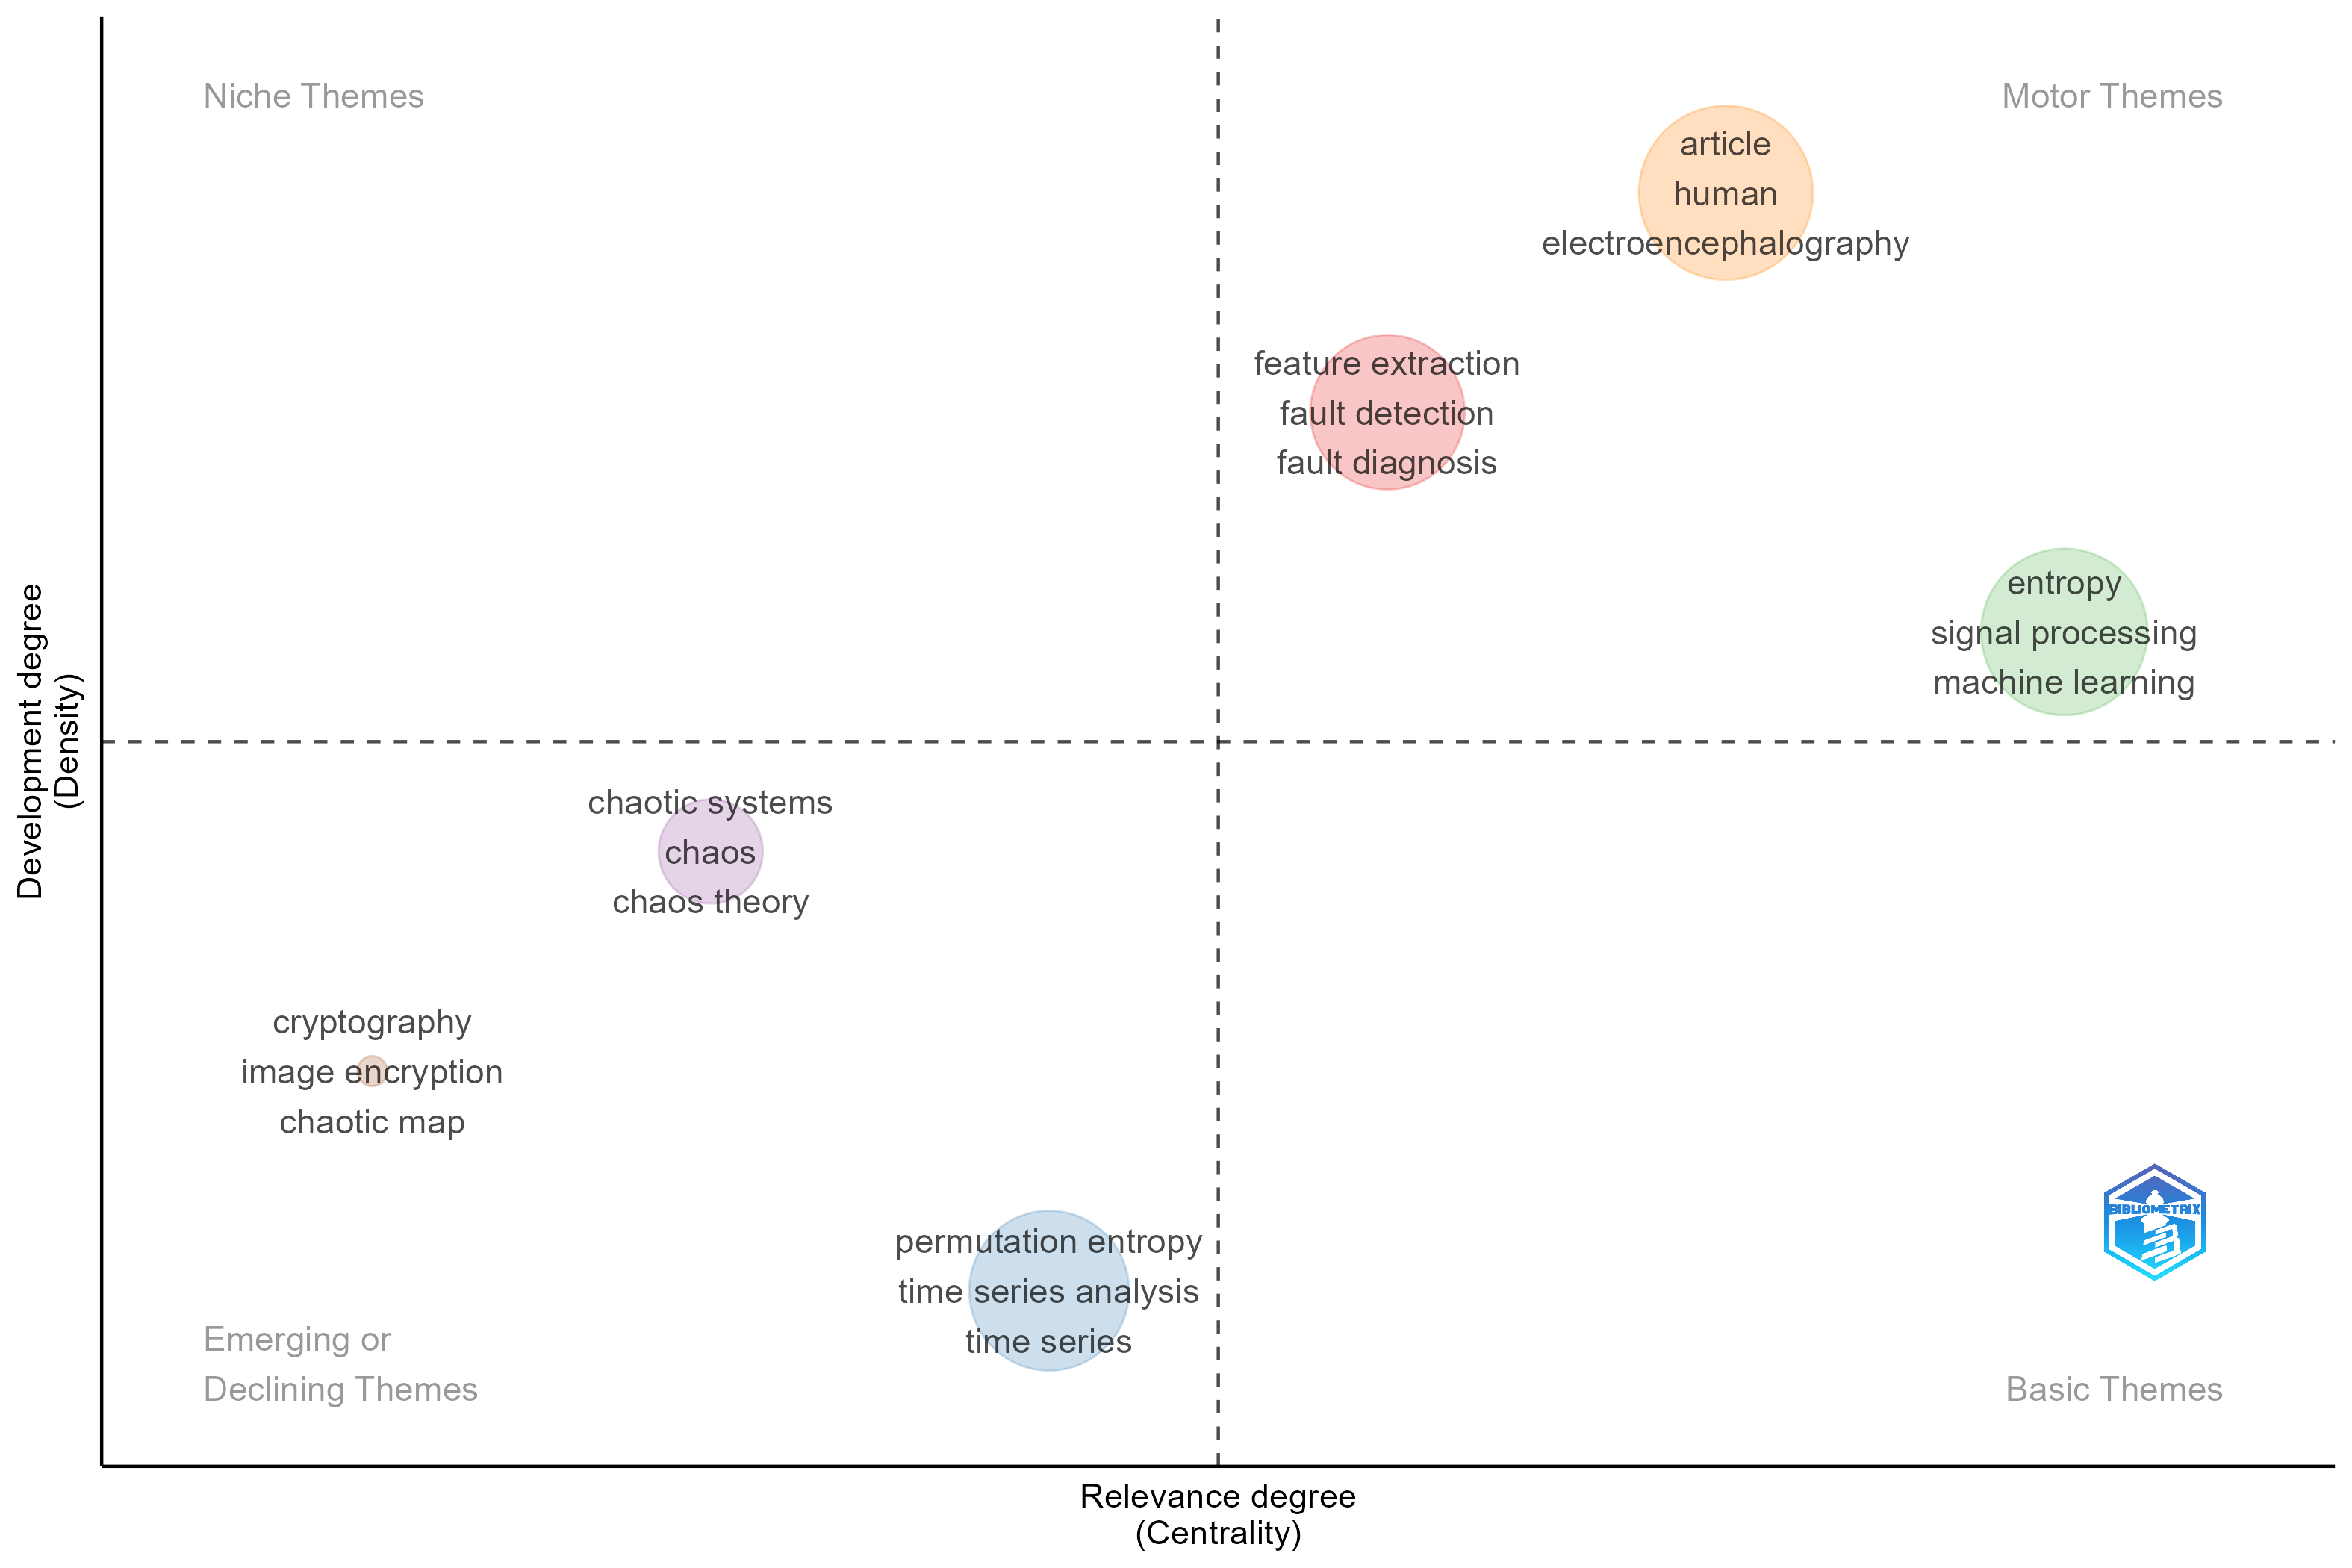
\includegraphics[width=\textwidth]{ThematicMap}
	\caption{The Thematic Map generated by Bibliometrix.}
	\label{fig:ThematicMap}
\end{figure}

The map is divided into four quadrants based on two dimensions: centrality (relevance) and density (development). The quadrant representing Motor Themes includes topics such as entropy, signal processing, and machine learning, indicating well-developed and highly interconnected areas of research. Basic Themes include permutation entropy and time series analysis, which are foundational topics in the field and closely align with the focus of this thesis. Niche Themes such as chaos theory and chaotic systems represent specialized subfields, while Emerging or Declining Themes like cryptography and image encryption reflect peripheral or potentially declining research interests. This thematic analysis provides a clear framework for situating the present research within the broader academic landscape, emphasizing both its theoretical foundation and its relevance to contemporary research trends.

\subsection{Factorial Map Analysis}
To identify the visual map of the main research topics based on the keywords, we analyze the factorial map.

\begin{figure}[H]
	\centering
	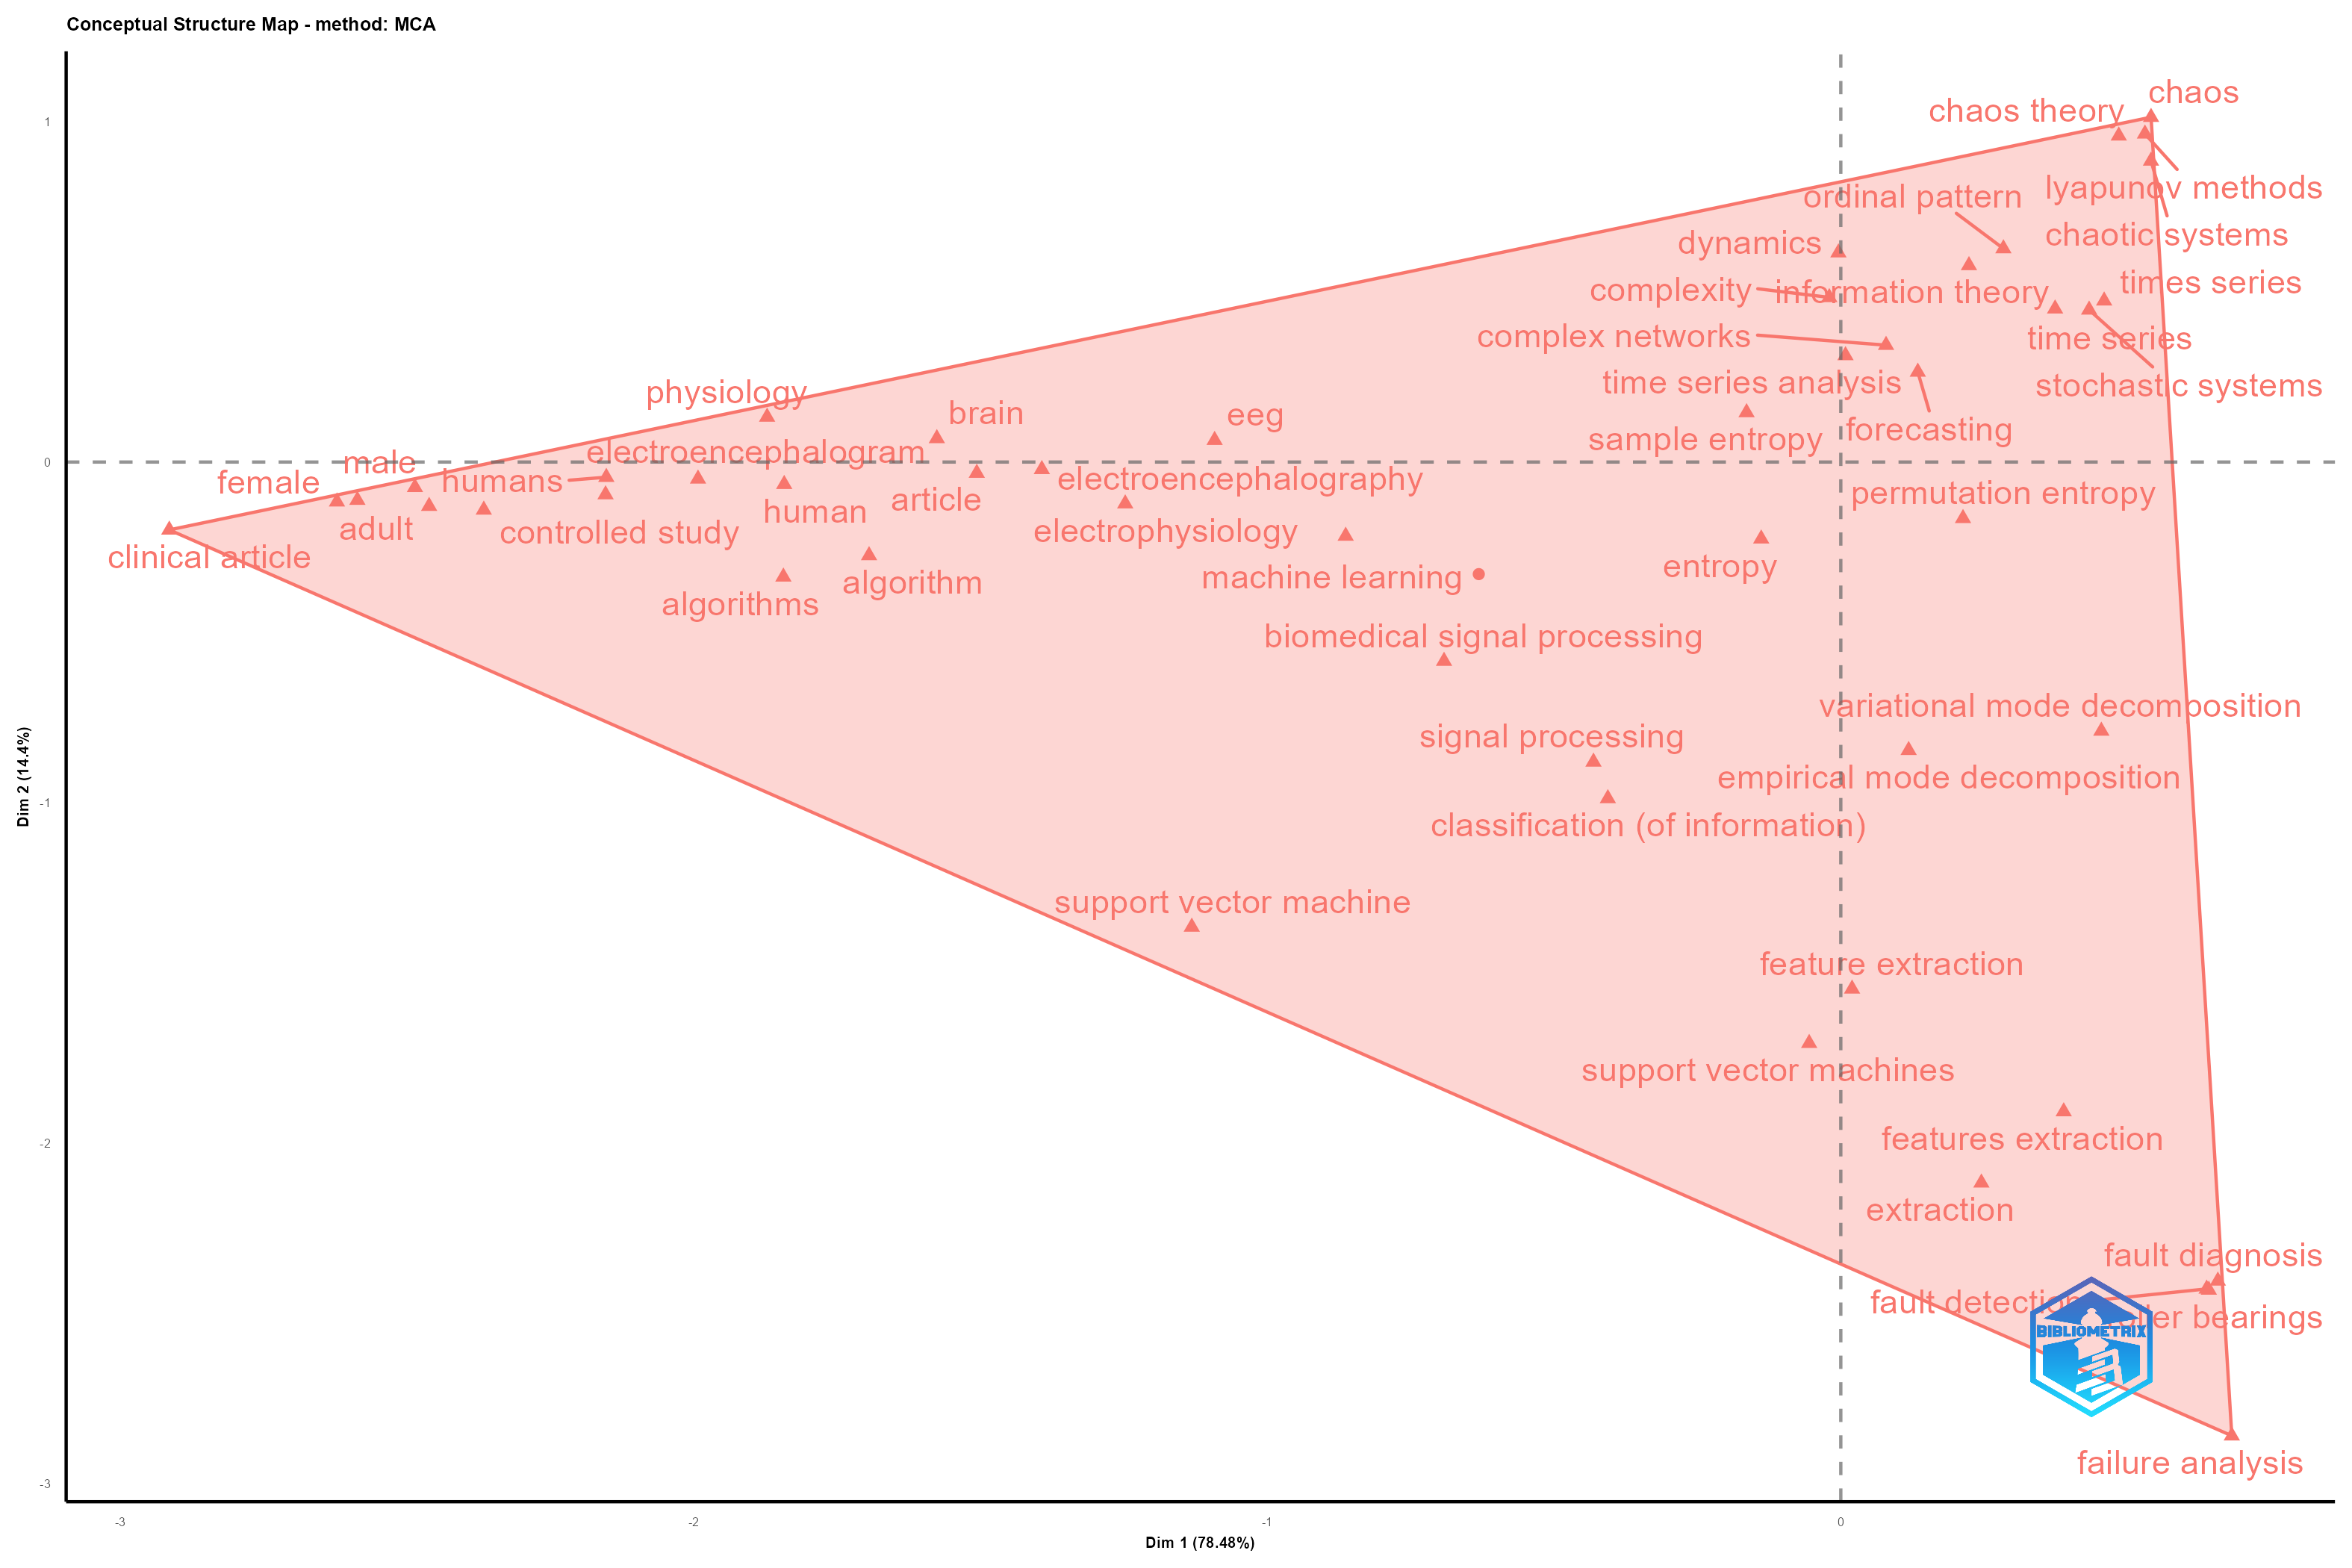
\includegraphics[width=0.9\textwidth]{FactorialMap}
	\caption{Factorial map generated by Bibliometrix.}
	\label{fig:factorialMap}
\end{figure}
%%% ACF Interpret: what do the axes mean? What does the point size encode?

The factorial map in Figure \ref{fig:factorialMap} reveals four major conceptual clusters:

The first cluster (upper right) includes theoretical concepts such as chaos theory, chaotic systems, Lyapunov methods, ordinal pattern, information theory, complex networks, and permutation entropy, forming the theoretical core of the research area.

The second cluster (lower right) includes practical applications such as feature extraction, empirical mode decomposition, variational mode decomposition, fault diagnosis, fault detection, and failure analysis, emphasizing the applied relevance of complexity-based time series analysis.

The third cluster (center) comprises terms related to biomedical signal processing and machine learning, including biomedical signal processing, EEG, support vector machine, classification, and machine learning, indicating the multidisciplinary applications of entropy measures.

A fourth, smaller cluster (left) includes clinical and physiological study keywords such as clinical article, controlled study, adult, male, female, humans, and physiology.

The factorial map thus provides further evidence of the diverse applications and theoretical development surrounding ordinal patterns and complexity measures, supporting the originality and relevance of the present research.

%\textcolor{red}{MAKE YOUR CONCLUSIONS HERE. WHICH TOPICS AND WHY?}
\subsection{Conclusion and Justification of Research Focus}

Based on the systematic literature review conducted using the Scopus-indexed references, it is evident that the research landscape surrounding ordinal patterns and complexity measures encompasses both theoretical foundations and a wide range of practical applications. Our proposed research strategically positions itself at the intersection of these domains. 
%%% ACF Is this true? !!!
The primary objective is to explore the feature extraction capabilities of ordinal patterns and apply complexity-based time series clustering for fault detection in rotating machinery, using publicly available ball bearing datasets.

The bibliometric analysis further highlights the multifaceted nature of this research area. The identified clusters illustrate a strong theoretical backbone, rooted in concepts such as ordinal patterns and permutation entropy, while also revealing a significant focus on real-world applications in fault diagnosis and failure analysis. Moreover, the presence of biomedical signal processing and machine learning within the intellectual structure underscores the versatility and broad applicability of complexity-based approaches across disciplines. However, since biomedical applications fall outside the scope of our research focus, we do not include a literature review on that area.

Furthermore, clinical and physiological study keywords indicate a notable research focus involving ordinal patterns and permutation entropy. However, as this area falls outside the scope of our research, it has also been excluded from the literature review.

%%% ACF !!! The chapter ends withtout providing teh information it promised at the beginning: the topics 


